% Grossmont College -- Chem 141 Lab 4: Redox Reactions - The Activity Series
% Cameron Carroll
% March 2014


\documentclass[fleqn,titlepage]{article}

\renewcommand*\rmdefault{ppl}

\usepackage[version=3]{mhchem} % Package for chemical equation typesetting
\usepackage{tabu}
\usepackage{wasysym}
\usepackage{listings}
\usepackage{scrextend}
\lstset{language=Matlab}
\usepackage{multirow}

% set 1" margins on 8.5" x 11" paper
% top left is measured from 1", 1"
\topmargin 0in
\oddsidemargin 0in
\evensidemargin 0in
\headheight 0in
\headsep 0in
\topskip 0in
\textheight 9in
\textwidth 6.5in

\usepackage{graphicx} % Required for the inclusion of images

\setlength\parindent{0pt} % Removes all indentation from paragraphs

\renewcommand{\labelenumi}{\alph{enumi}.} % Make numbering in the enumerate environment by letter rather than number (e.g. section 6)

%\usepackage{times} % Uncomment to use the Times New Roman font

%----------------------------------------------------------------------------------------
% DOCUMENT INFORMATION
%----------------------------------------------------------------------------------------

\begin{document}

\begin{titlepage}
  \mbox{}\\[1.25cm]
  \textbf{\LARGE Cameron Carroll \\ Grossmont College}\\[2.25cm]
  \begin{center}
    \textbf{\huge Lab 4: \\ Redox Reactions - The Activity Series}\\[2.50cm]
  \end{center}
  \textbf{\LARGE Professor: Martin Larter \\ Chemistry 141-0692} \\
  \vfill
  \center{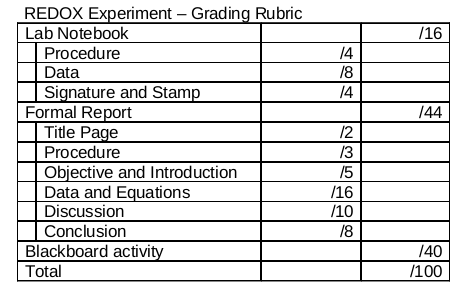
\includegraphics{./rubic_redox}}
  \center{\textbf{\LARGE Performed --} {\LARGE March 4, 2014}}
  \center{\textbf{\LARGE Submitted --} {\LARGE March 4, 2014}}
\end{titlepage}

%----------------------------------------------------------------------------------------
% SECTION 1
%----------------------------------------------------------------------------------------
\section*{Procedure}
\begin{itemize}
  \item  \textbf{Referenced From:} \\
    \begin{addmargin}[1em]{1em}
      Lehman, J. (Et al), `Redox Reactions - The Activity Series' \\
      Grossmont College, Chemistry 141 Lab Manual, 6th edition, pp 51-56 \\
      El Cajon, California
    \end{addmargin}
\end{itemize}

%----------------------------------------------------------------------------------------
% SECTION 2
%----------------------------------------------------------------------------------------
\section*{Objective}
  \paragraph{} This experiment investigates the relative reactivity of various elements by attempting reactions between them.These observations are then used to construct an activity series, showing which elements are most reactive and therefore are the strongest reducing agents.

%----------------------------------------------------------------------------------------
% SECTION 3
%----------------------------------------------------------------------------------------
\section*{Introduction}
  \paragraph{} Oxidation state, a hypothetical bookkeeping device where atoms are assigned charges as if all of their bonds were ionic, is used to determine relative reactivity and whether a reaction will occur. The process of oxidation corresponds to an increase in oxidation state, and also to a loss of electrons. Reduction is the opposite: gain of electrons and decrease in oxidation state. An oxidation agent is a substance which oxidizes something else -- By the nature of a redox (oxidation-reduction) reaction, something else (the oxidation agent itself) must be reduced. Again, a reduction agent is the opposite in the pair, a chemical which reduces and is itself oxidized.

%----------------------------------------------------------------------------------------
% SECTION 4
%----------------------------------------------------------------------------------------
\newpage
\section*{Data}
\textsc{Notes:}
\begin{description}
  \item[Blank Observations] Correspond to no reaction criteria... no color change, heat, gas formation, or precipitate formation.\\[-.5cm]
  \item[Ox.] Element Oxidized\\[-.5cm]
  \item[Red.] Element Reduced\\[-.5cm]
  \item[OA] Oxidizing Agent
  \item[MA] More Active Element
\end{description}
  \begin{tabular}{|c|p{3.7cm}|c|c|c|c|c|}
    \hline
    Reactants & Observations & Net Reaction & Ox. & Red. & OA & MA \\
    \hline
    \ce{Cu} \& \ce{Zn^{2+}} & & NO RXN & & & & Zn \\
    \hline
    \ce{Cu} \& \ce{Fe^{2+}} & & NO RXN & & & & Fe \\
    \hline
    \ce{Zn} \& \ce{Cu^{2+}} & Zn strip turned black had bubbles on it, later broke apart. & \ce{Zn(s) + Cu^{2+}(aq) -> Zn^{2+}(aq) + Cu(s)} & Zn & Cu & Cu & Zn \\
    \hline
    \ce{Zn} \& \ce{Fe^{2+}} & Green solution turns clear. & \ce{Zn(s) + Fe^{2+}(aq) -> Zn^{2+}(aq) + Fe(s)} & Zn & Fe & Fe & Zn \\
    \hline
    \ce{Fe} \& \ce{Cu^{2+}} & Blue solution turns green. & \ce{Fe(s) + Cu^{2+}(aq) -> Fe^{2+}(aq) + Cu(s)} & Fe & Cu & Cu & Fe \\
    \hline
    \ce{Fe} \& \ce{Zn^{2+}} & & NO RXN & & & Cu & Zn \\
    \hline
    \ce{Cu} \& \ce{H+} & & NO RXN & & & Cu & H \\
    \hline
    \ce{Zn} \& \ce{H+} & Bubbles visible on Zn strip. & \ce{Zn(s) + 2H+(aq) -> Zn^{2+}(aq) + H2(g)} & Zn & H & H & Zn \\
    \hline
    \ce{Fe} \& \ce{H+} & Steel wool loses color and has visible bubbles. & \ce{Fe(s) + 2H+(aq) -> Fe^{2+}(aq) + H2(g)} & Fe & H & H & Fe \\
    \hline
    \ce{I2} \& \ce{Br-} & Hexane layer held a pinkish color, indicating nonpolar \ce{I2}. & NO RXN & & & & I \\
    \hline
    \ce{Br2} \& \ce{I-} & Hexane layer held a pinkish color again, indicating \ce{I2}. & \ce{Br2(aq) + 2I^-(aq) -> 2Br^-(aq) + I2(aq)} & I & Br & Br & I \\
    \hline
    \ce{Fe^{3+}} \& \ce{Br-} & & NO RXN & & & & Fe \\
    \hline
    \ce{Fe^{3+}} \& \ce{I-} & Solution darkens to red. & \ce{2Fe^{3+}(aq) + 2I^-(aq) -> 2Fe^{2+}(aq) + I2(aq)} & I & Fe & Fe & I \\
    \hline
    \ce{Cu} \& \ce{Br2} & Adding \ce{NH3} turns solution blue, indicating \ce{Cu(NH3)4^{2+}}. Also, adding \ce{AgNO3} yields a precipitate. & \ce{Cu + Br2 -> Cu^{2+} + 2Br-} & Cu & Br & Br & Cu \\
    \hline
    \ce{Cu} \& \ce{I2} & Adding \ce{AgNO3} may have yielded a precipitate, but \ce{NH3} didn't turn the solution blue. & NO RXN & & & & \\
    \hline
  \end{tabular}
%----------------------------------------------------------------------------------------
% SECTION 5
%----------------------------------------------------------------------------------------
\section*{Discussion}
\paragraph{} There wasn't enough data to build a complete and definite activity series. Foremost, \ce{Fe^{3+}} cannot be placed in the primary activity series, $Zn > I > Fe > H > Cu > Br$, because we only know that it's less reactive than I and more reactive than Br. We would need to react it against Fe, H and Cu to find it a place in the table. \\
Also, in the last step, the combination of elemental Cu and \ce{I2}, I was unable to determine relative reactivity. They were both in elemental form and there was no reaction, yielding no information.s
s
%----------------------------------------------------------------------------------------
% SECTION 6
%----------------------------------------------------------------------------------------
\section*{Conclusion}
  \paragraph{} Two series are actually a better representation of the data than one...
  \center{$Zn > I > Fe > H > Cu > Br$}
  \center{$I > \ce{Fe^{3+}} > Br$}



\end{document}